\subsection{Evaluation of an Android Device in a WiFi Network}
The communication package bundling the network specific classes was exported with the help of eclipse as a \textit{.jar} file. This file was added as a library to the Android project, ensuring a seamless reuse of the already written parts. 

\subsubsection{Android App as client}
\begin{figure}[H]
	\centering
	\begin{subfigure}{.49\textwidth}
		\centering
		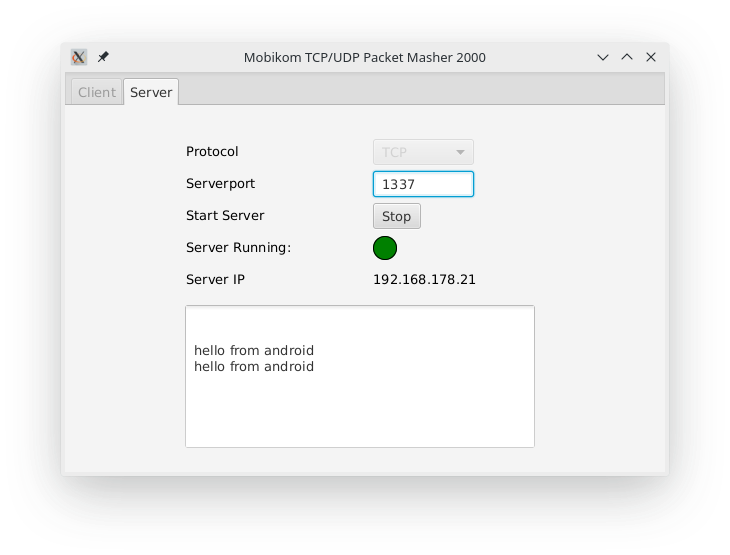
\includegraphics[width=1\linewidth]{images/task3/subtask2/serverTCPNEW.png}
		\caption{The server on the JVM, TCP}
	\end{subfigure}
	\begin{subfigure}{.49\textwidth}
		\centering
		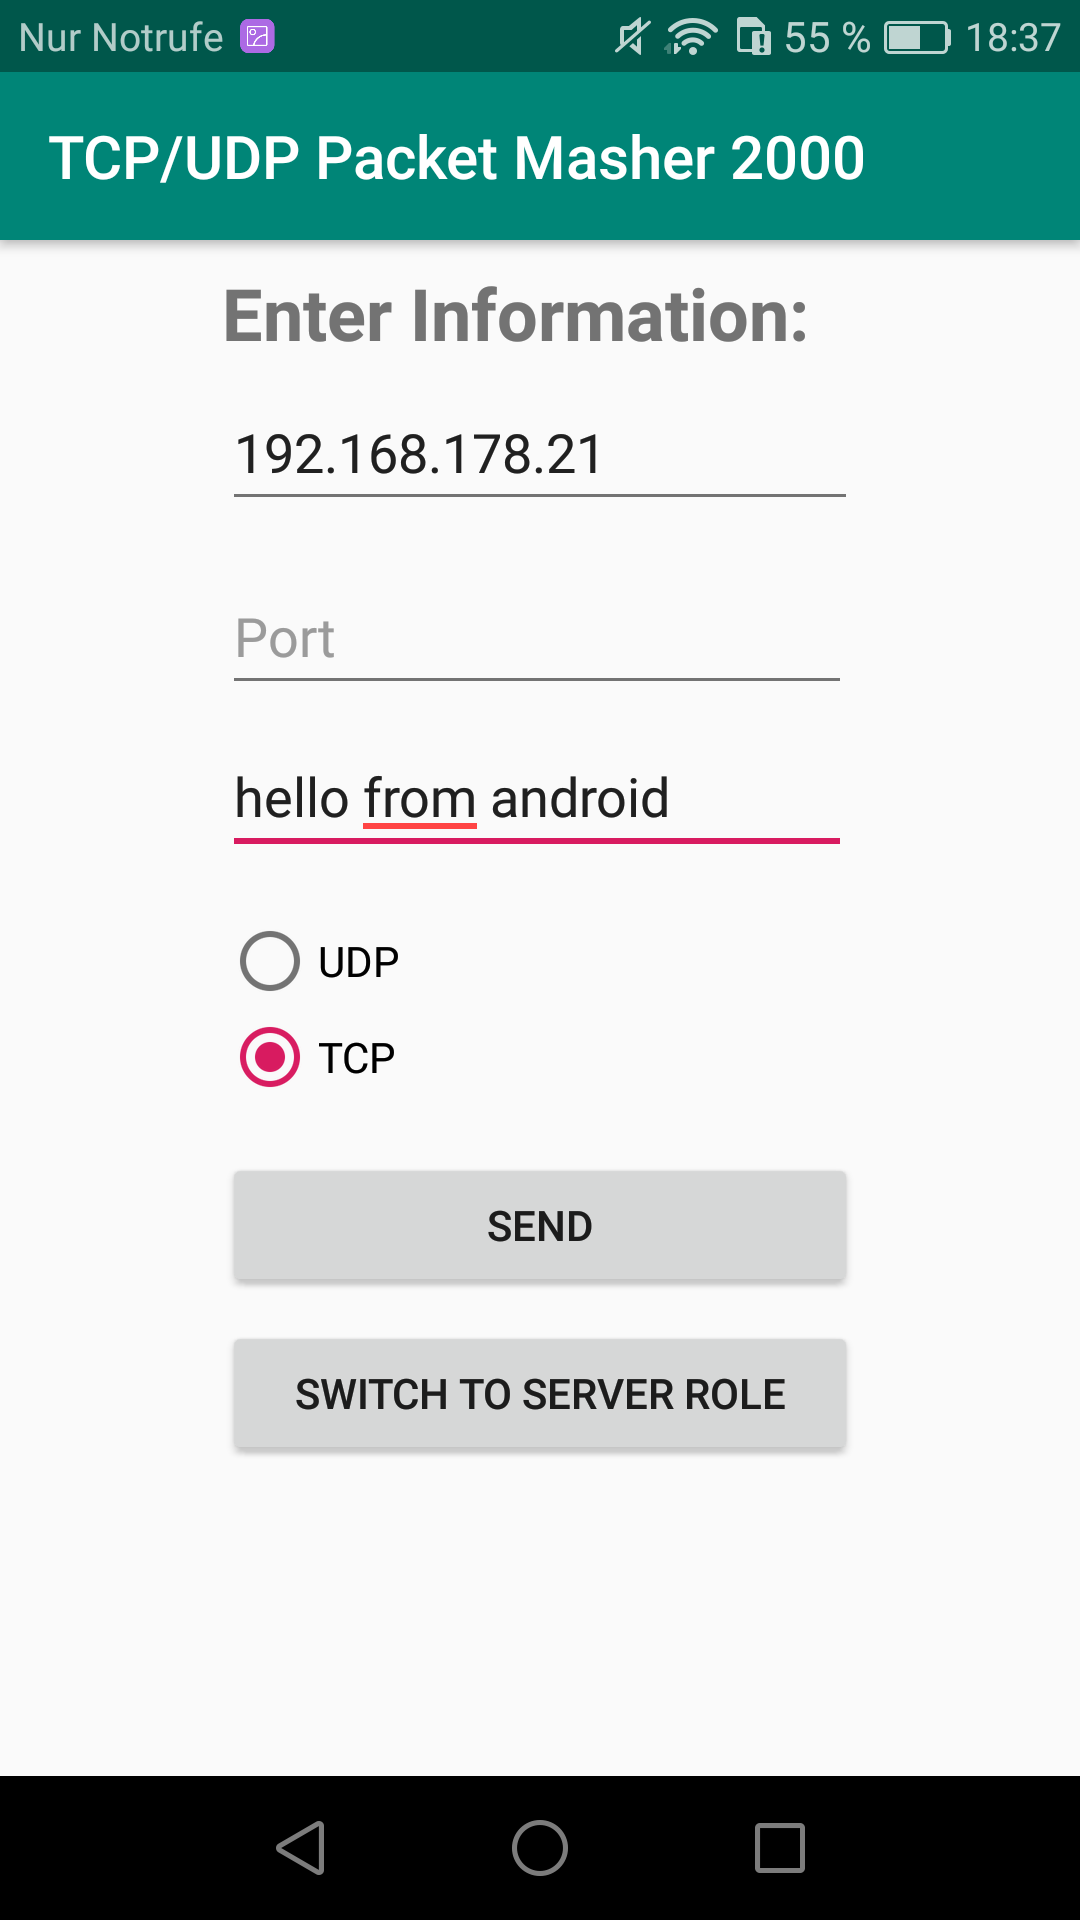
\includegraphics[width=0.74\linewidth]{images/task3/subtask2/android/clientTCP.png}
		\caption{The client interface on Android}
	\end{subfigure}%
	\caption{Server on the JVM, Android as client, TCP}
	\label{fig:androidClientTCP}
\end{figure}



\begin{figure}[H]
	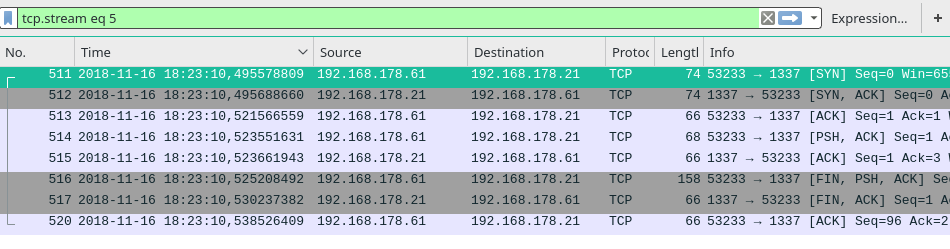
\includegraphics[width=1\linewidth]{images/task3/subtask2/wireshark/jvmServerTCP.png}
	\caption{Wireshark traces where Android App acts as a TCP server}
	\label{fig:wire2}
\end{figure}

\texttt{....sr..communication.Message...........L..messaget..Ljava/lang/String;xpt..hello from android}



\begin{figure}[H]
	\centering
	\begin{subfigure}{.49\textwidth}
		\centering
		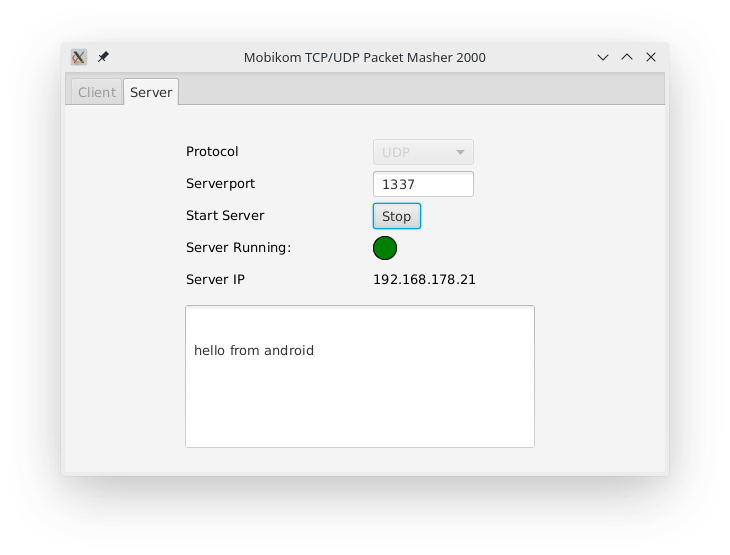
\includegraphics[width=1\linewidth]{images/task3/subtask2/serverUDPNEW.png}
		\caption{The server on the JVM, UDP}
	\end{subfigure}
	\begin{subfigure}{.49\textwidth}
		\centering
		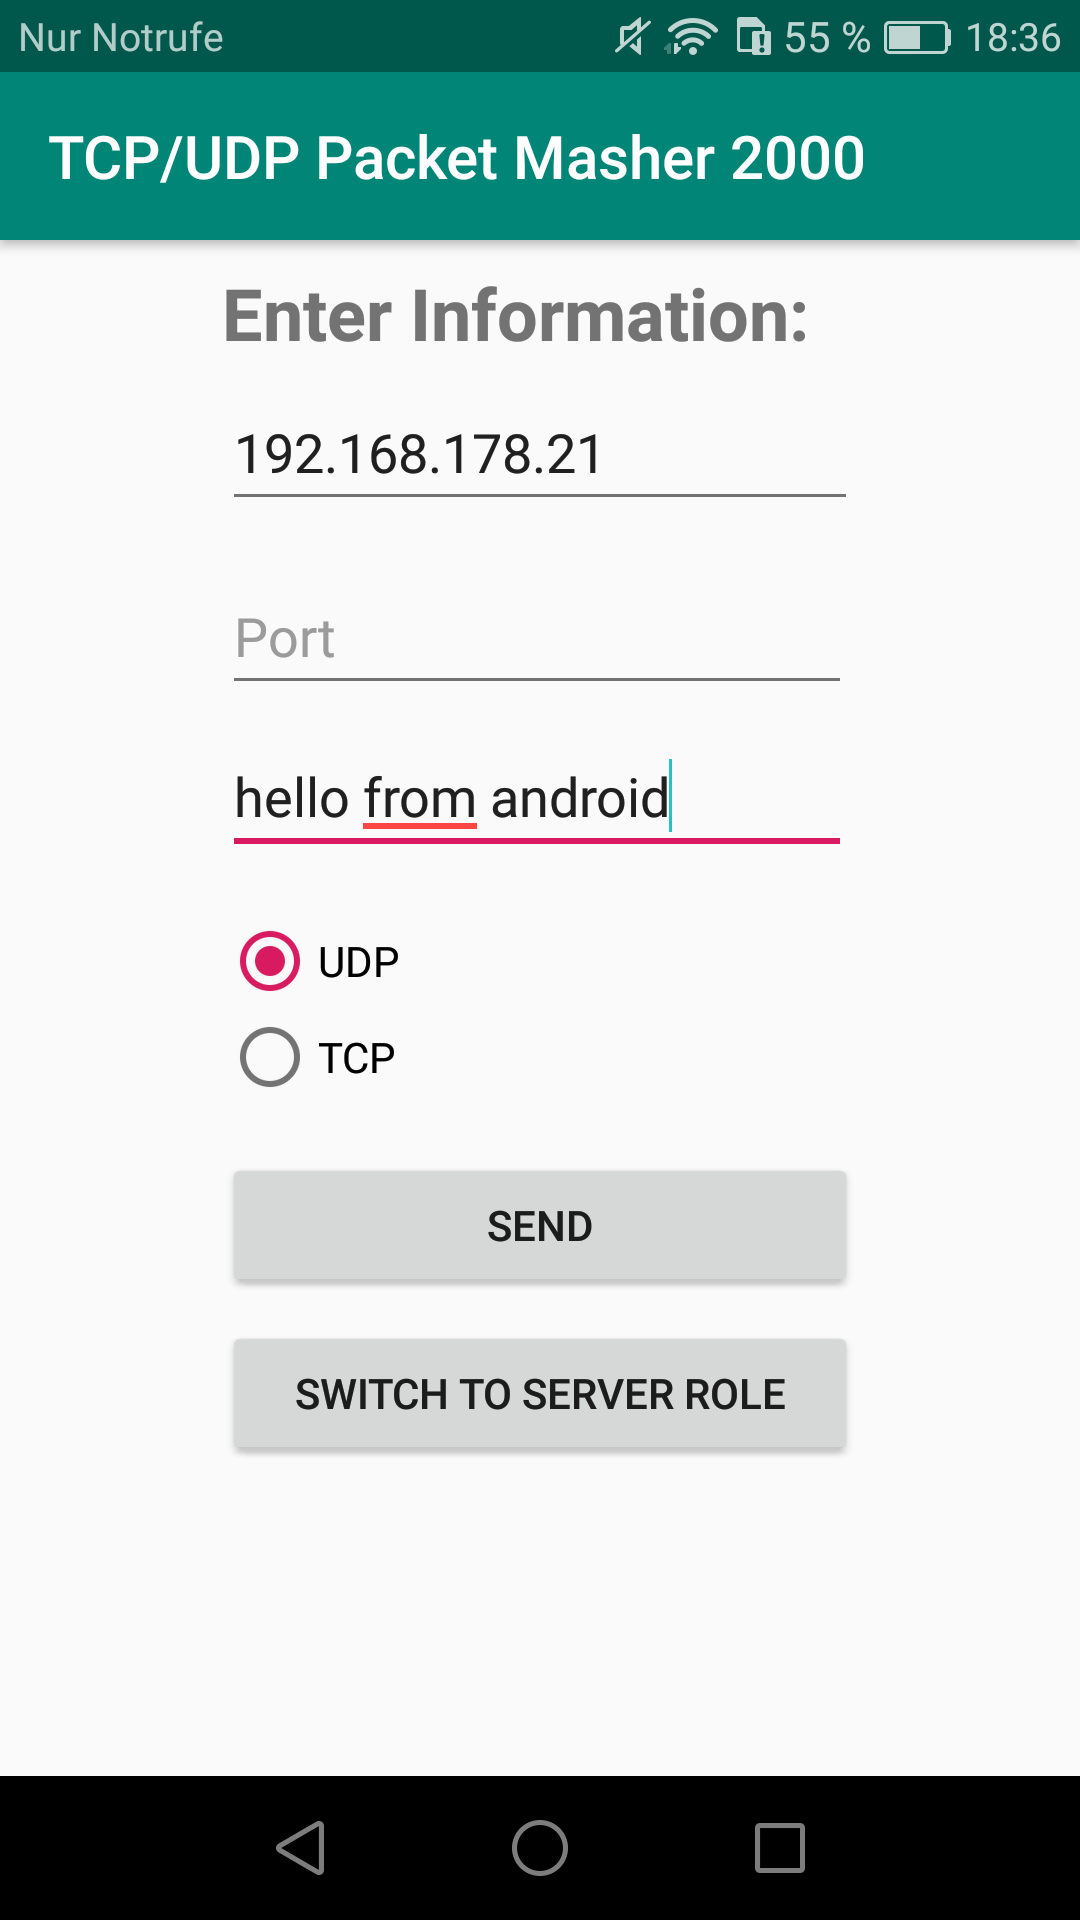
\includegraphics[width=0.74\linewidth]{images/task3/subtask2/android/clientUDP.png}
		\caption{The client interface on Android}
	\end{subfigure}%
	\caption{Server on the JVM, Android as client, UDP}
	\label{fig:androidClientUDP}
\end{figure}

\begin{figure}[H]
	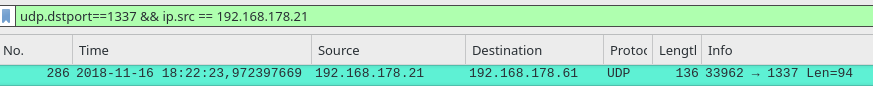
\includegraphics[width=1\linewidth]{images/task3/subtask2/wireshark/jvmServerUDP.png}
	\caption{Wireshark traces where Android App acts as a TCP server}
	\label{fig:wire3}
\end{figure}


\texttt{....sr..communication.Message...........L..messaget..Ljava/lang/String;xpt..hello from android}


\subsubsection{Android App as server}

\begin{figure}[H]
	\centering
	\begin{subfigure}{.49\textwidth}
		\centering
		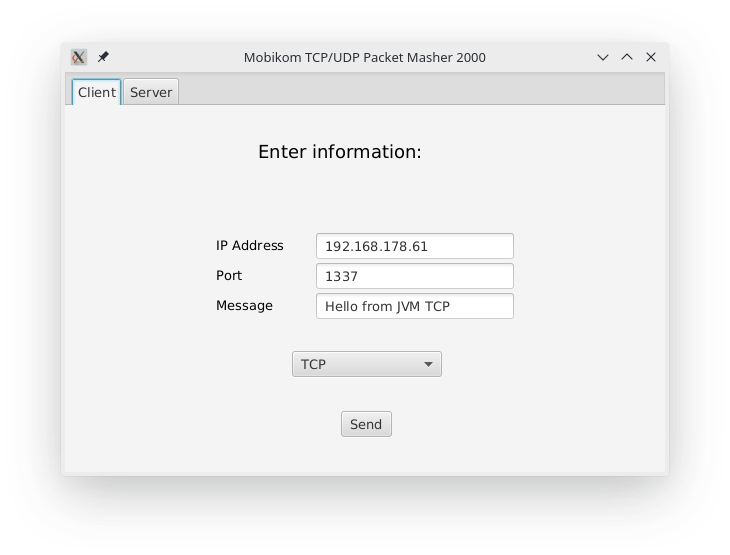
\includegraphics[width=1\linewidth]{images/task3/subtask2/clientTCPNEW.png}
		\caption{Client on the JVM, TCP}
	\end{subfigure}
	\begin{subfigure}{.49\textwidth}
		\centering
		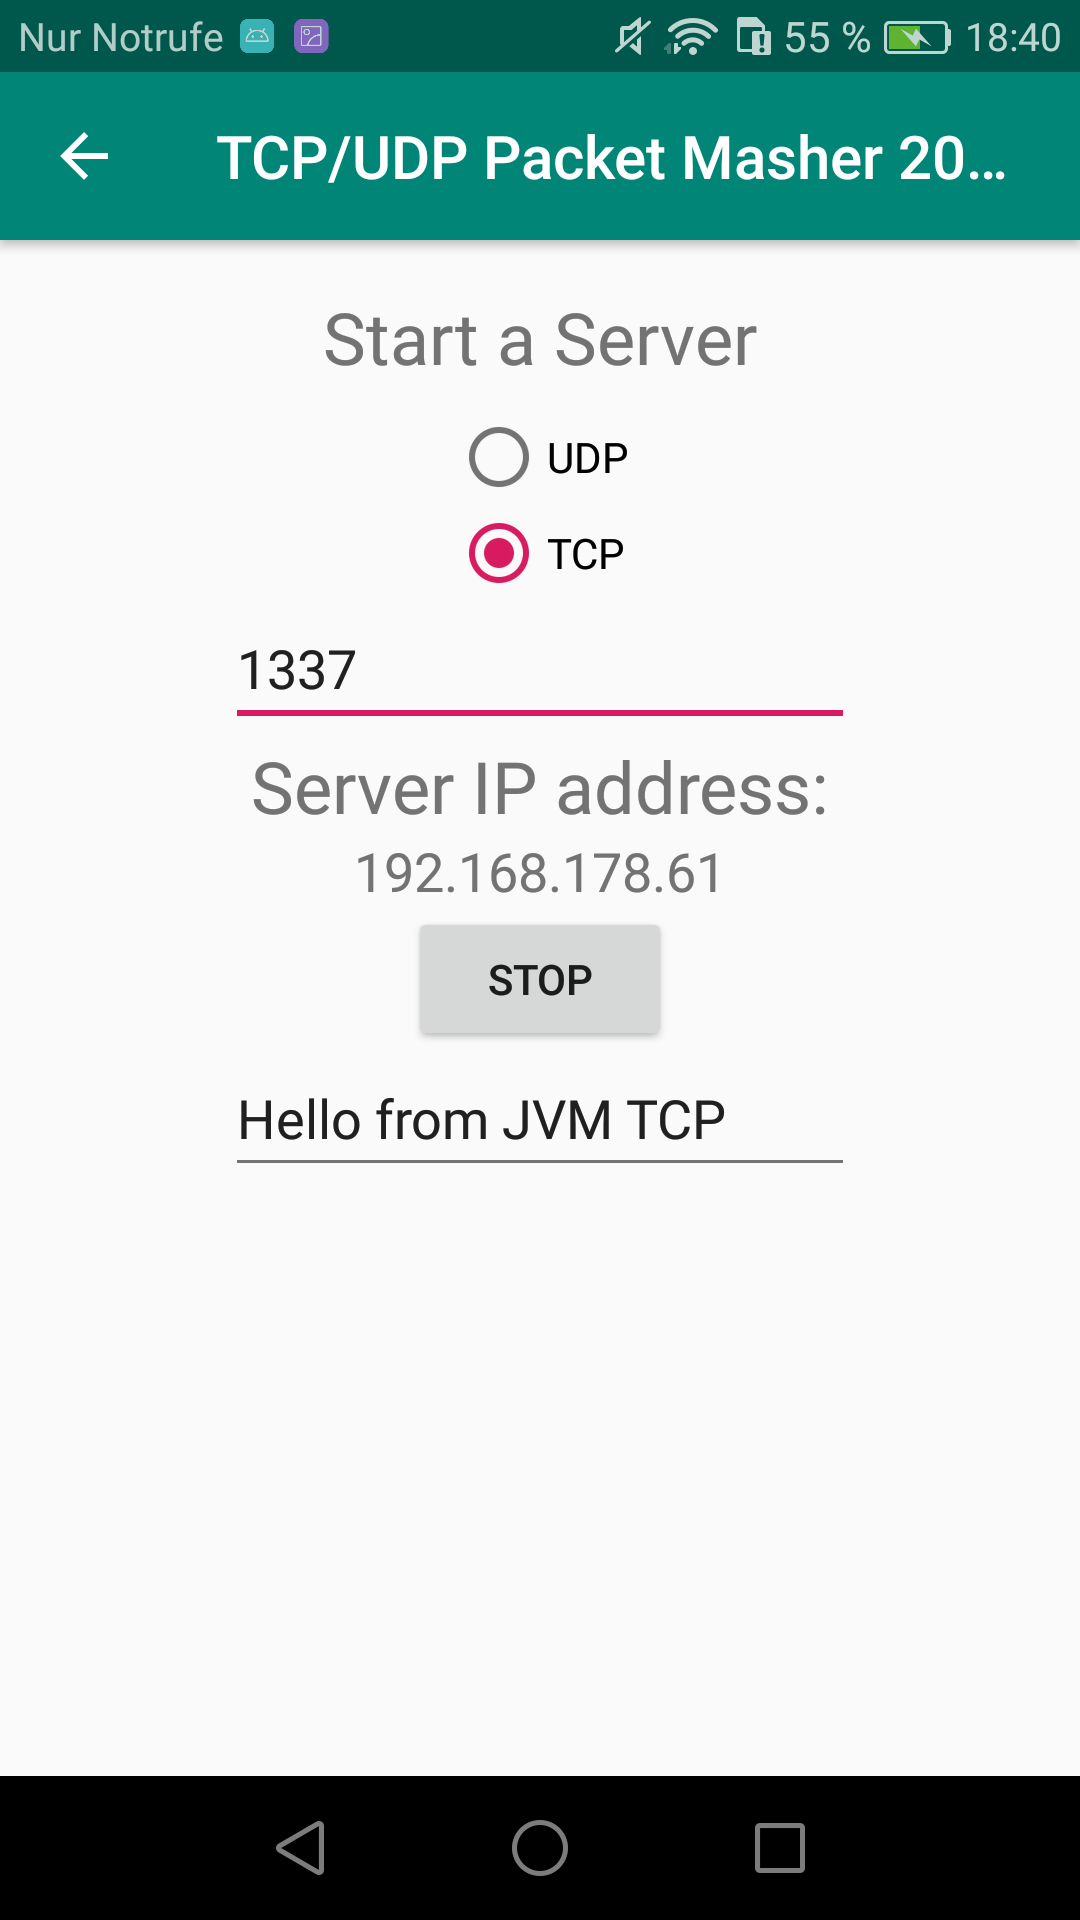
\includegraphics[width=0.74\linewidth]{images/task3/subtask2/android/serverTCP.png}
		\caption{The server interface with JavaFX}
	\end{subfigure}%
	\caption{Server on Android, JVM application as client, TCP}
	\label{fig:androidServerTCP}
\end{figure}


\begin{figure}[H]
	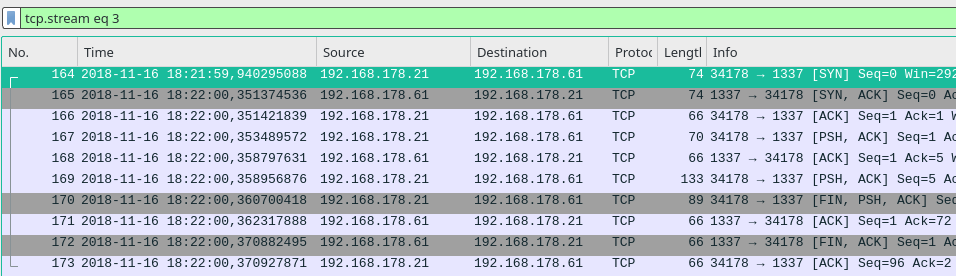
\includegraphics[width=1\linewidth]{images/task3/subtask2/wireshark/androidServerTCP.png}
	\caption{Wireshark traces where Android App acts as a TCP server}
	\label{fig:wire4}
\end{figure}



\texttt{....sr..communication.Message...........L..messaget..Ljava/lang/String;xpt..Hello from JVM TCP}


\begin{figure}[H]
	\centering
	\begin{subfigure}{.49\textwidth}
		\centering
		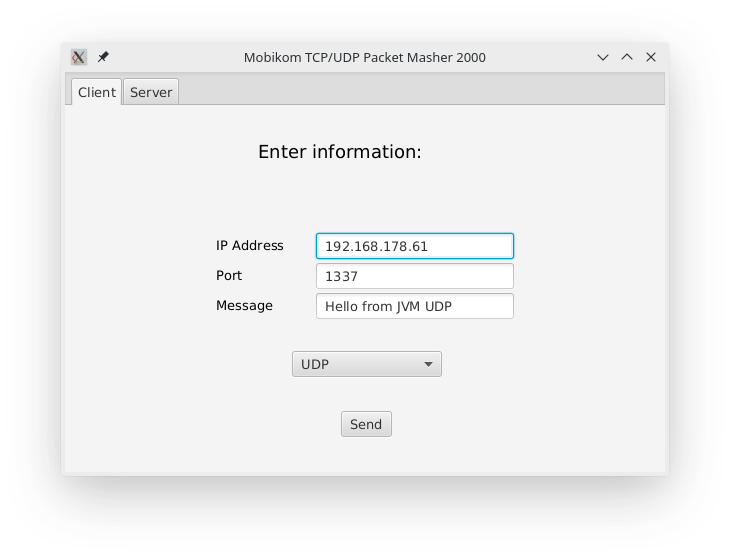
\includegraphics[width=1\linewidth]{images/task3/subtask2/clientUDPNEW.png}
		\caption{Client on the JVM, UDP}
	\end{subfigure}
	\begin{subfigure}{.49\textwidth}
		\centering
		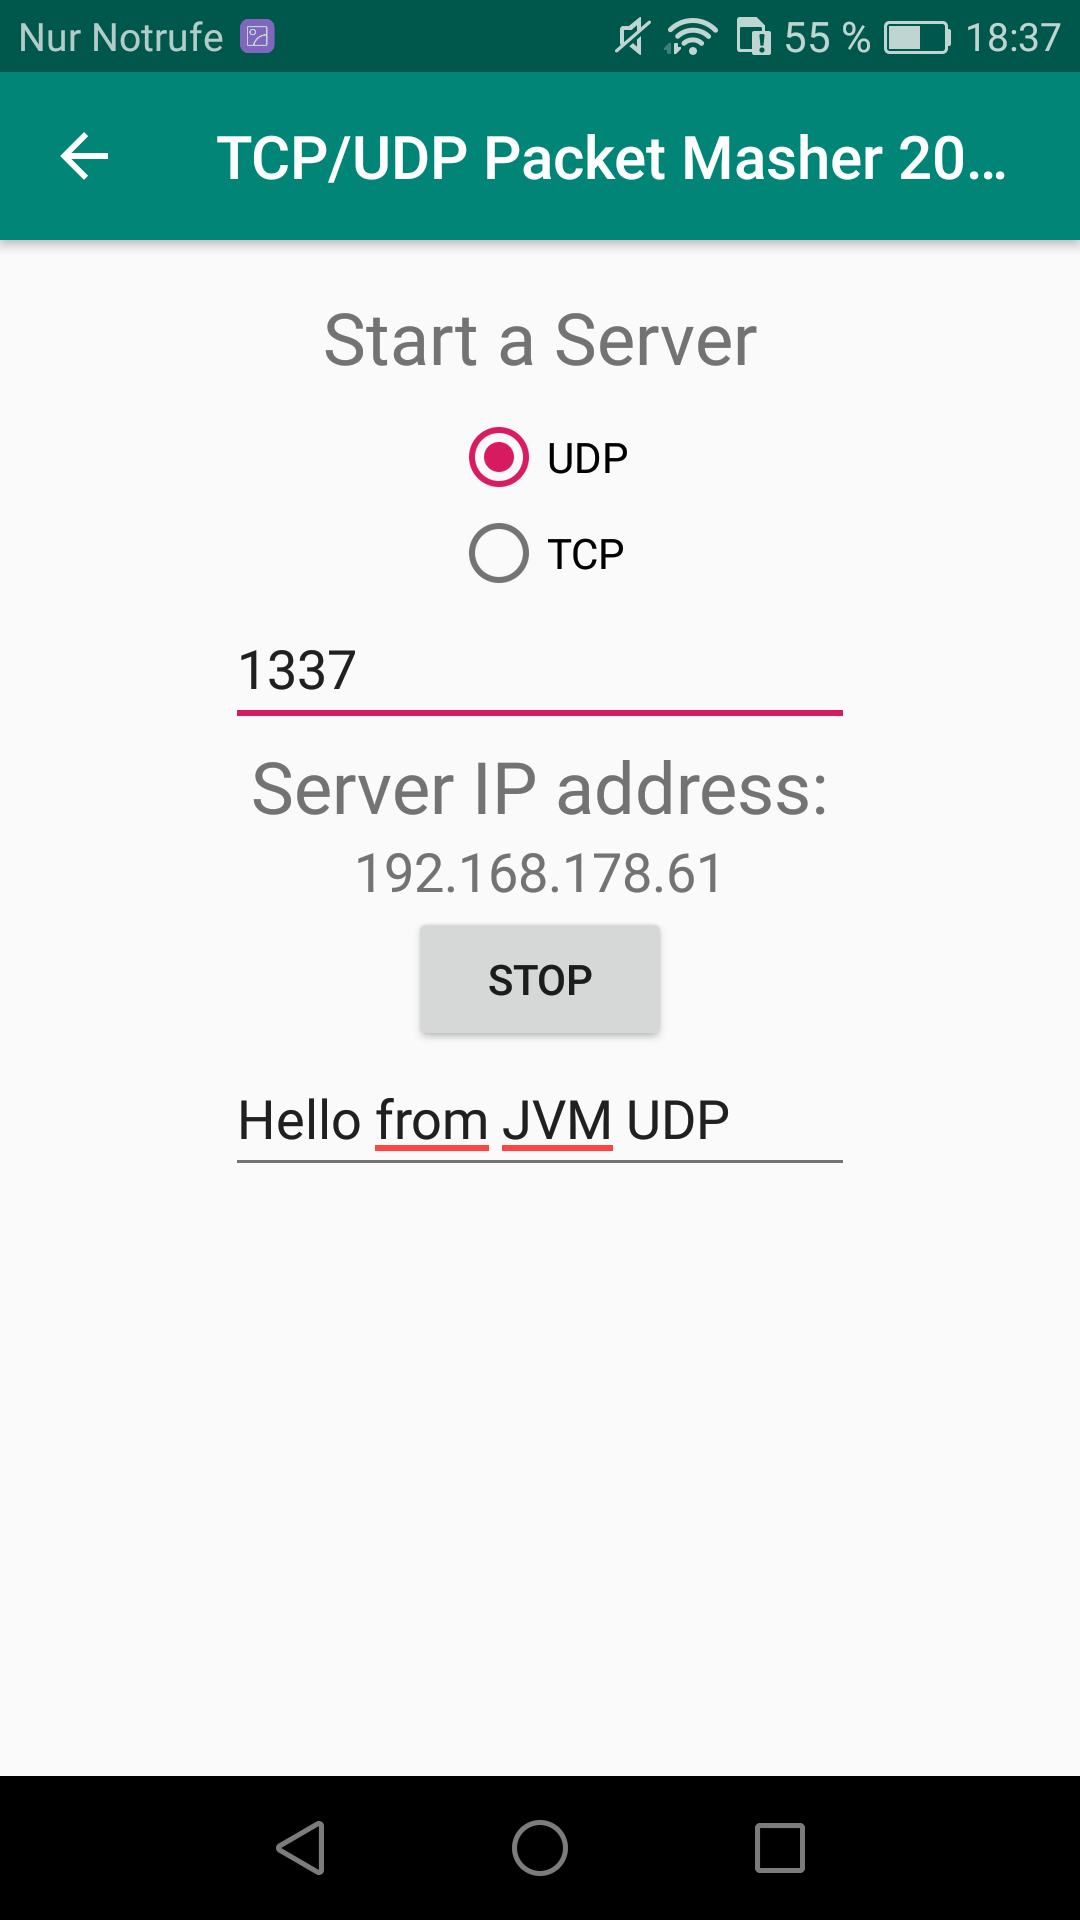
\includegraphics[width=0.74\linewidth]{images/task3/subtask2/android/serverUDP.png}
		\caption{The server interface with JavaFX}
	\end{subfigure}%
	\caption{Server on Android, JVM application as client, UDP}
	\label{fig:androidServerUDP}
\end{figure}

\begin{figure}[H]
	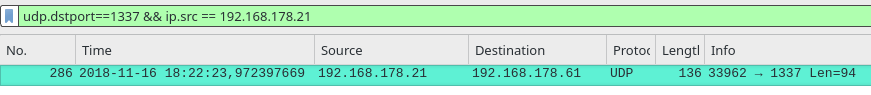
\includegraphics[width=1\linewidth]{images/task3/subtask2/wireshark/androidServerUDP.png}
	\caption{Wireshark traces where Android App acts as a TCP server}
	\label{fig:wire5}
\end{figure}

\texttt{....sr..communication.Message...........L..messaget..Ljava/lang/String;xpt..Hello from JVM UDP}